\documentclass[]{book}

\usepackage{import}
\usepackage{preamble}

\begin{document}

\noindent BECA / Huson / 11.1 IB Math SL \hspace{2in} Name:\\*
23 October 2017
\begin{center}
{\Large Test Corrections: Functions and Quadratics}\\
\textit{Redo the graphs on which you missed any points. Due Thursday.}
\end{center}

%\vspace{0.2 cm}
\subsection*{Sketching a quadratic function}
Answer on lined paper and use this sheet for the graph.

\begin{enumerate}


\item   Given $f(x)=-(x-3)^2+16$
\begin{enumerate}
    \item Write down the vertex of the function as an ordered pair.
    \item Write down the equation of the axis of symmetry.
    \item Expand the function from vertex form to standard form, $ax^2+bx+c \text{ where } a, b, c \;  \epsilon \; \mathbb{R}$.
    \item Write down the value of $f(0)$. Explain what this represents on the graph.
    \item Hence factor the function. Write down the roots.
    \item Sketch the function, labeling the intercepts with values and the vertex as an ordered pair. Show the axis of symmetry as a dotted line and label it with its equation.
\begin{figure}[!ht]
    \flushright
    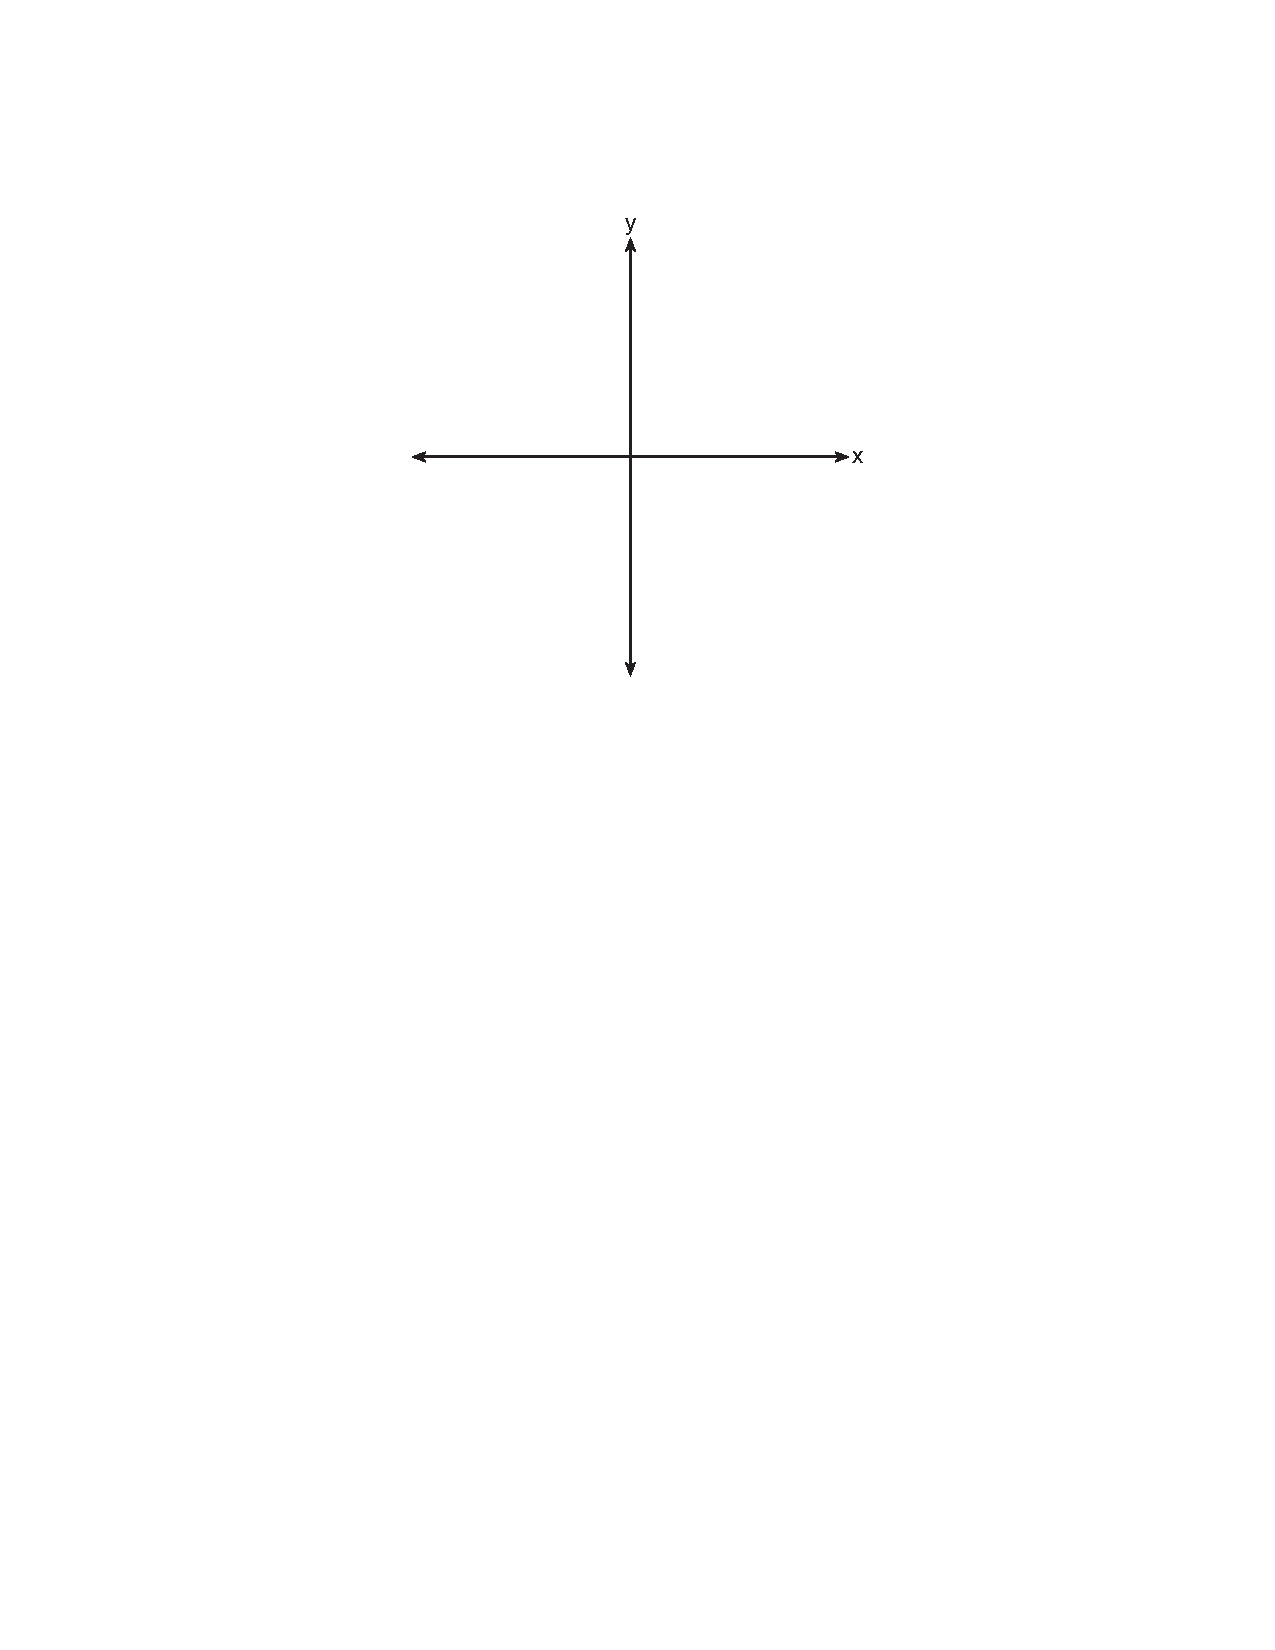
\includegraphics[width=0.6\textwidth]{simple-axes.pdf}
\end{figure}

    \item Write down the domain and range of the function.\\*[10pt]
\end{enumerate}


\newpage
\subsection*{Graphing quadratics}
Answer on lined paper. Graph the function on the grid shown below.
\item Given the function $f(x)=-x^2-x+6$. 
\begin{enumerate}
    \item Write down the $y$-intercept.
    \item State whether the parabola opens upward or downward. Explain how you know this from the function expressed in standard form.
    \item Express the function in factored form. Hence state the solutions to $f(x)=0$.
    \item Show that the axis of symmetry of the parabola is $x=-\frac{1}{2}$.
    \item Hence state the vertex as an ordered pair. 
    \item Graph the function. Mark the vertex as an ordered pair and label each intercept with its value. Plot the axis of symmetry as a dotted line and label it with its equation.
    \item Write down the domain and range of the function.
\end{enumerate}

\begin{figure}[!ht]
    \centering
    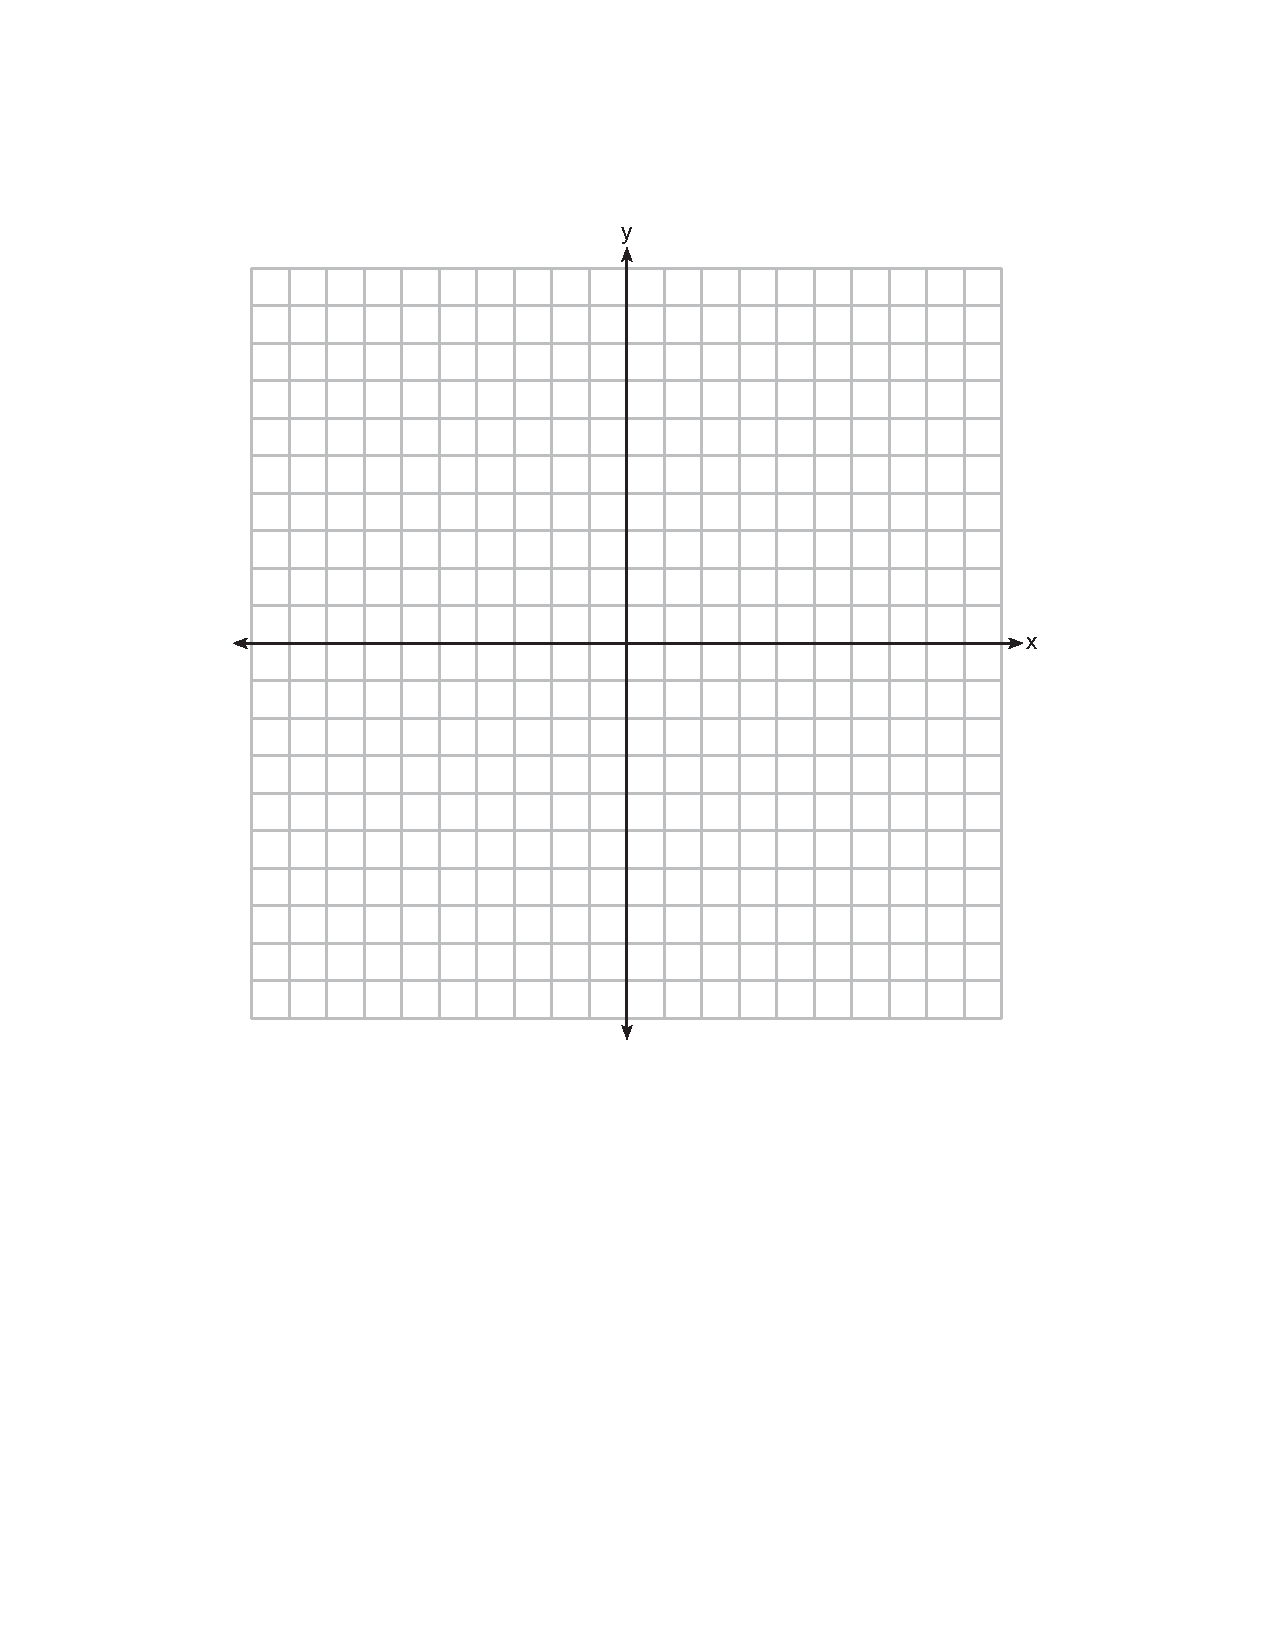
\includegraphics[width=0.75\textwidth]{regents-grid.pdf}
\end{figure}

\newpage
\item  
\begin{enumerate}
    \item Graph the parent function $f(x)=x^2$. Mark the point $P(3, f(3))$ on the graph
    \item The function $g(x)$ is the function $f$ after being translated to the right 5 and down 4. Graph $g$.
    \item Mark the point on the function $g$, $Q$, that represents the point $P$ after the translation.
\end{enumerate}

\begin{figure}[!ht]
    \centering
    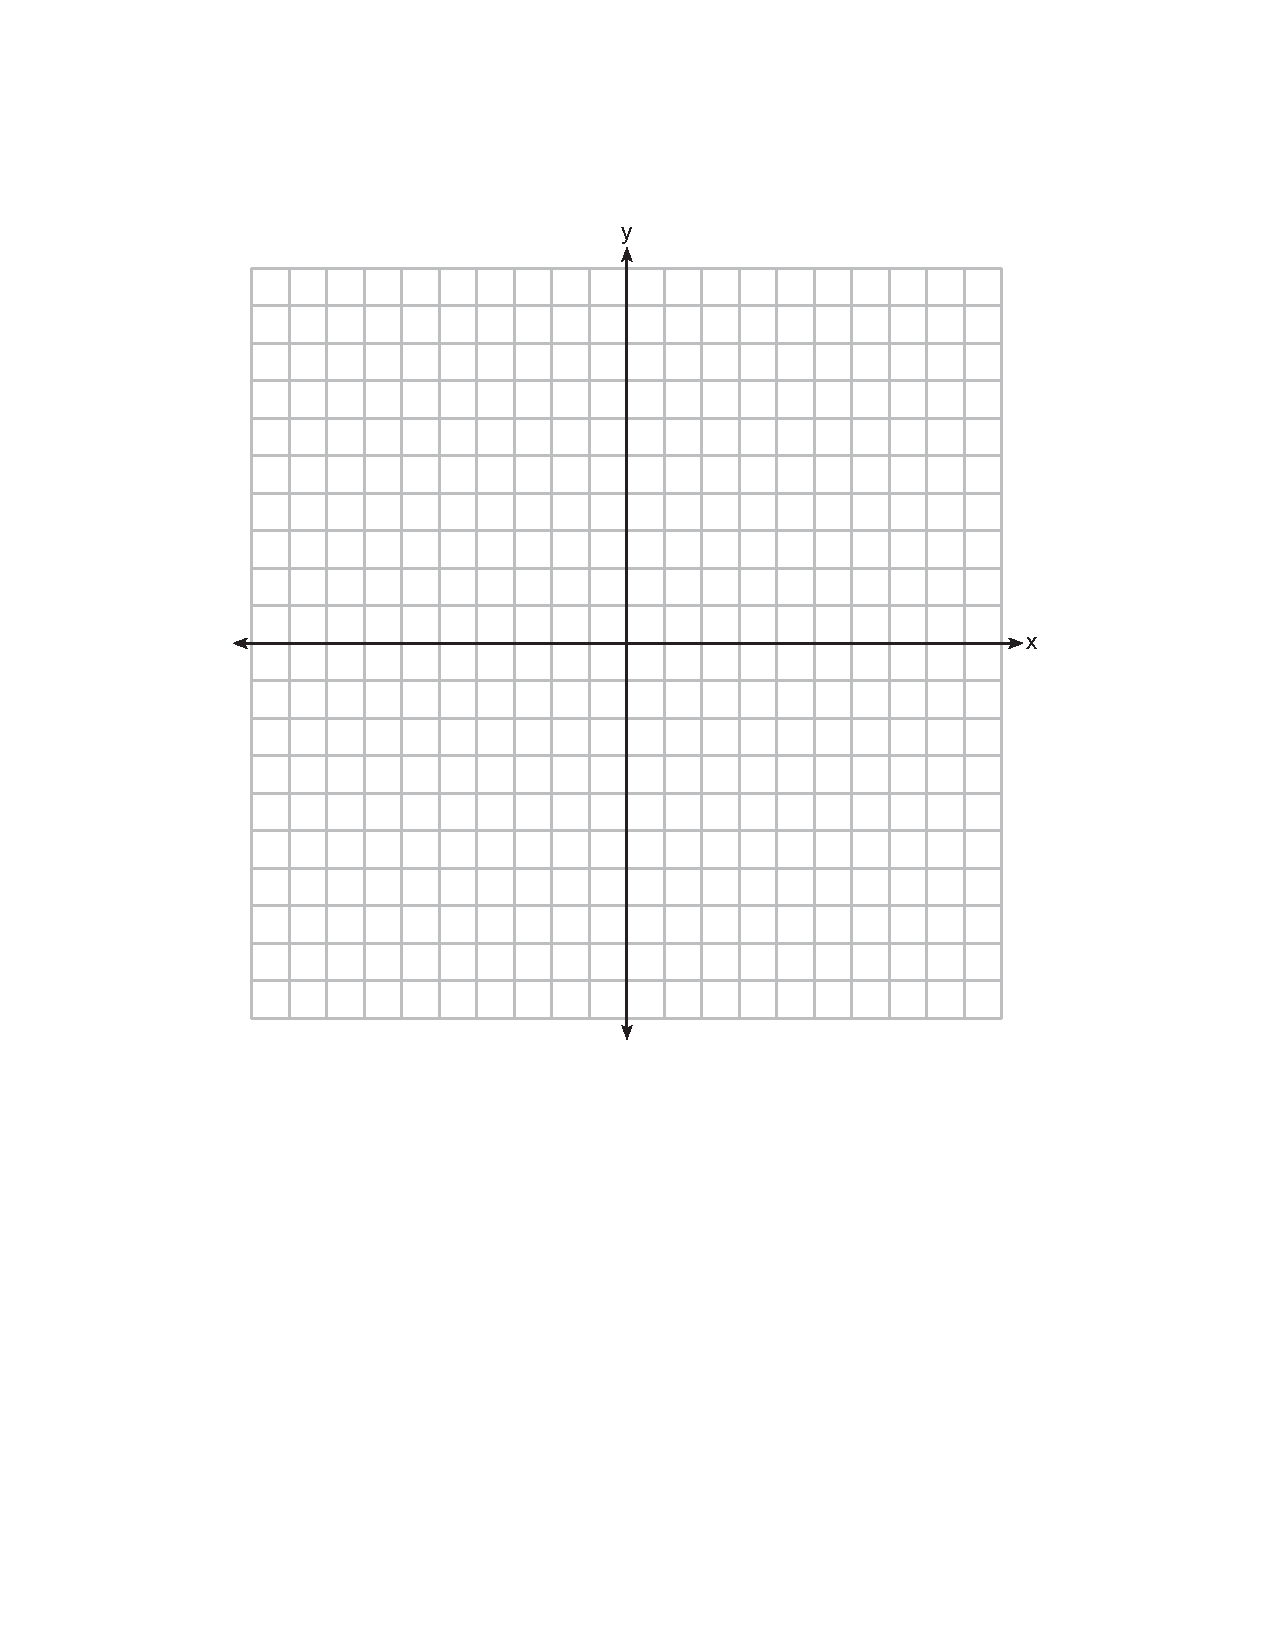
\includegraphics[width=0.75\textwidth]{regents-grid.pdf}
\end{figure}

\newpage
\subsection*{Model situations with quadratic functions}
\item The path of a diver is given by 
\[f(x)=-5x^2+12x+9\]
where $y$ is the height (in meters) and $x$ is time in seconds.\\*[5pt]
\begin{enumerate}
    \item On the grid below, graph the function over the domain where $x\geq 0$ and the range where $f(x) \geq 0$. Use a horizontal scale of 5 squares equals one second and vertical scale of 1 square equals one meter. Label the intercepts and vertex.
    \item What is the maximum height of the diver? Label the point on the graph with the work ``max.''\\*[30pt]
    \item What is the time when the diver enters the water? Label the point on the graph representing this with the word ``splash.''\\*[30pt]
\end{enumerate}

\begin{figure}[!ht]
    \flushright
    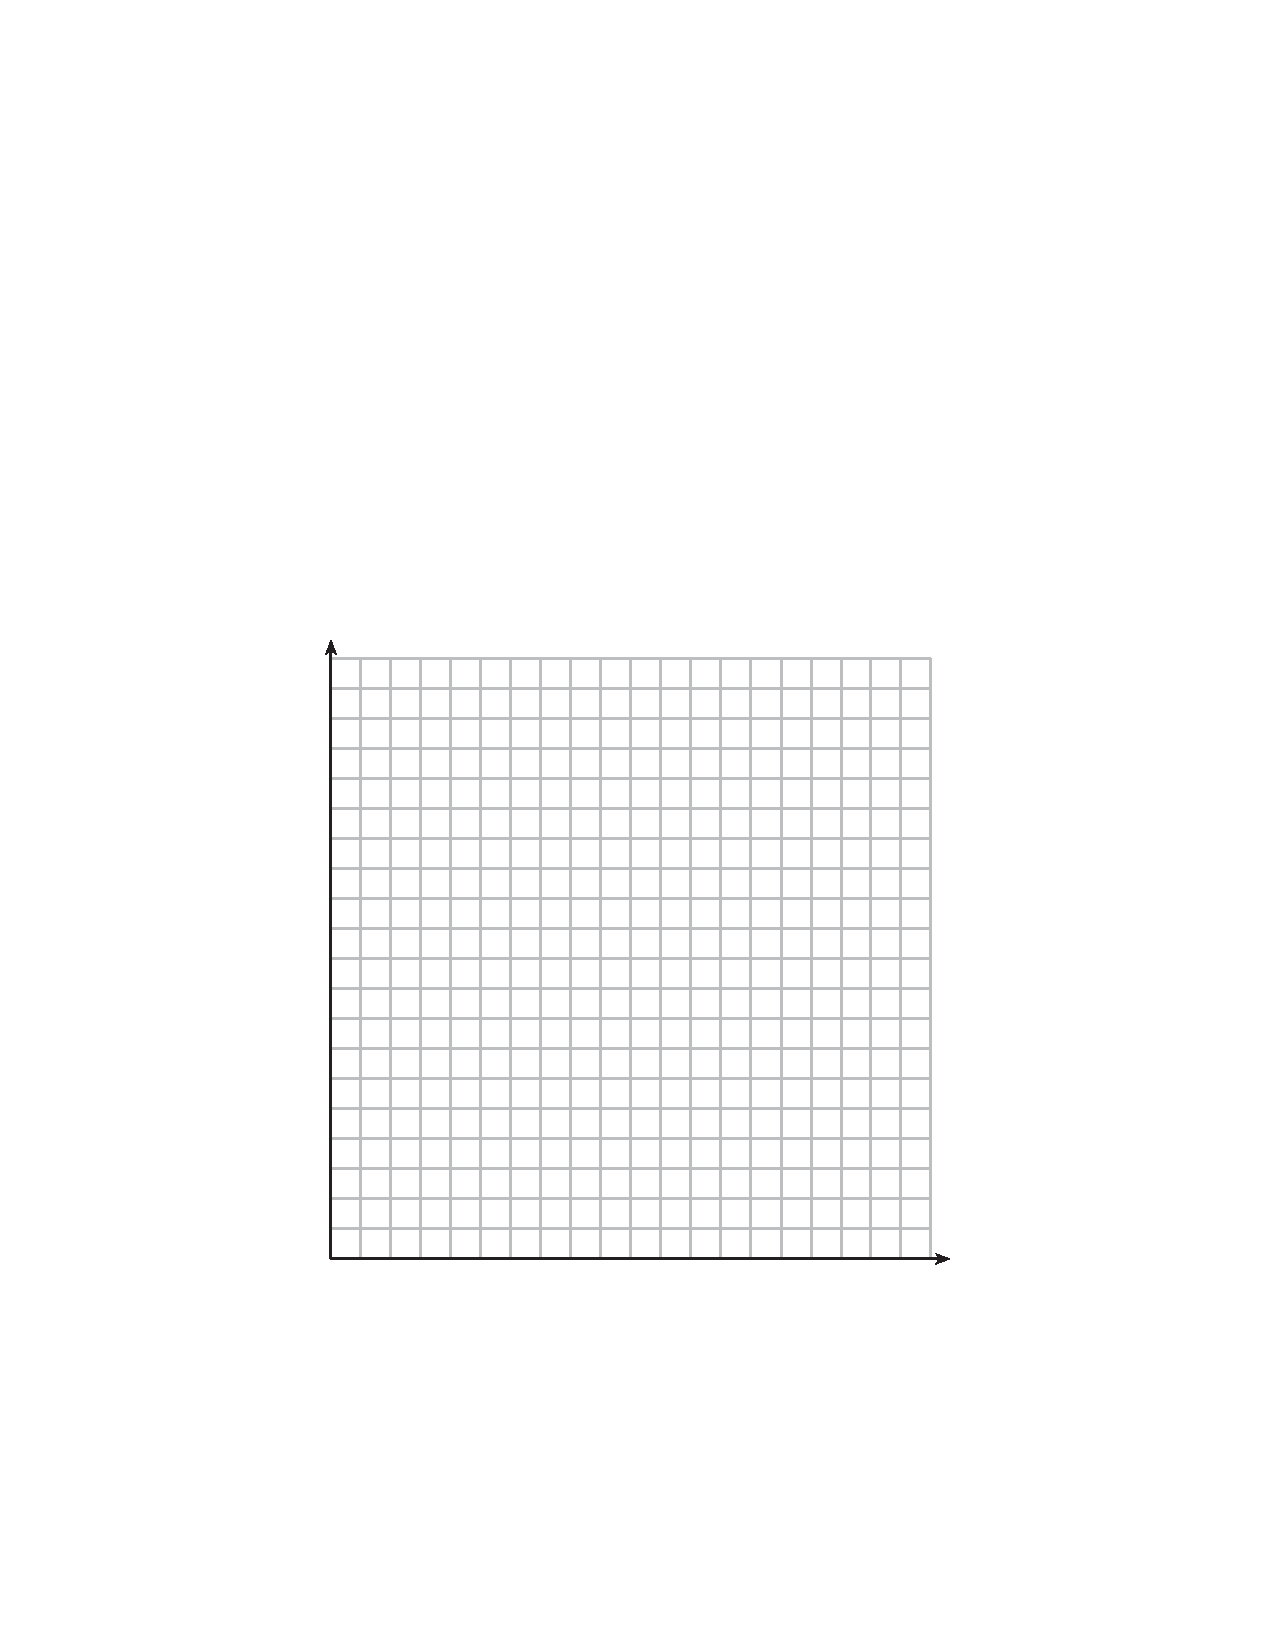
\includegraphics[width=0.65\textwidth]{1stQ-grid.pdf}
\end{figure}

\end{enumerate}

\end{document}